\chapter{Additional Design Diagrams}

\begin{longtable}{>{\raggedright\arraybackslash}p{0.28\textwidth}>{\raggedright\arraybackslash}p{0.26\textwidth}>{\raggedright\arraybackslash}p{0.32\textwidth}}
\caption{Supplementary diagrams and their implementation links.}\label{tab:appendix-diagrams}\\
\toprule
\textbf{Diagram} & \textbf{Purpose} & \textbf{Implementation connection}\\
\midrule
\endfirsthead
\toprule
\textbf{Diagram} & \textbf{Purpose} & \textbf{Implementation connection}\\
\midrule
\endhead
\texttt{layered-arch.tex} & System layers and trust boundaries & Web, worker, contracts, Supabase and provider-adapter separation.\\
\texttt{components.tex} & Component responsibilities and interfaces & Adapter, ingestion, graph, packet, verifier and reviewer components.\\
\texttt{dfd.tex} & Evidence and event flow & Provider delivery through normalization, persistence and downstream verification.\\
\texttt{verifier-loop.tex} & Bounded scope/verify/critic loop & \texttt{apps/worker/src/verifier/loop.ts}.\\
\texttt{autonomy-ladder.tex} & Human involvement by decision level & Reviewer findings, abstention and verdict gate.\\
\texttt{06\_state\_machines.tex} & Event, freshness and finding lifecycle & Duplicate handling, stale sources and review state transitions.\\
\texttt{05\_ingestion\_sequence.tex} & Source delivery sequence & Authentication, normalization, idempotency and reconciliation boundary.\\
\texttt{11\_deployment.tex} & Single-host deployment footprint & Containers, volumes, ports and the inbound/outbound boundary.\\
\texttt{erd.tex} & Relational evidence graph schema & Supabase nodes, edges, events, packets, verdicts and findings.\\
\texttt{anchor-reanchoring.tex} & Requirement-to-code anchoring & FR-22--FR-24 design and future commit-pinned anchors.\\
\bottomrule
\end{longtable}

\noindent Diagram sources are stored under
\texttt{docs/F26 FYP1 Mid Report LaTeX/diagrams/}. Abdullah's five diagrams
were consolidated by commit \texttt{7abdfc7}; Haaniah's state-machine and
ingestion diagrams are retained as supplementary evidence.

Figures~\ref{fig:ingestion-sequence}, \ref{fig:state-machines} and
\ref{fig:deployment} reproduce the three supplementary diagrams referenced
above.

\lsfigure{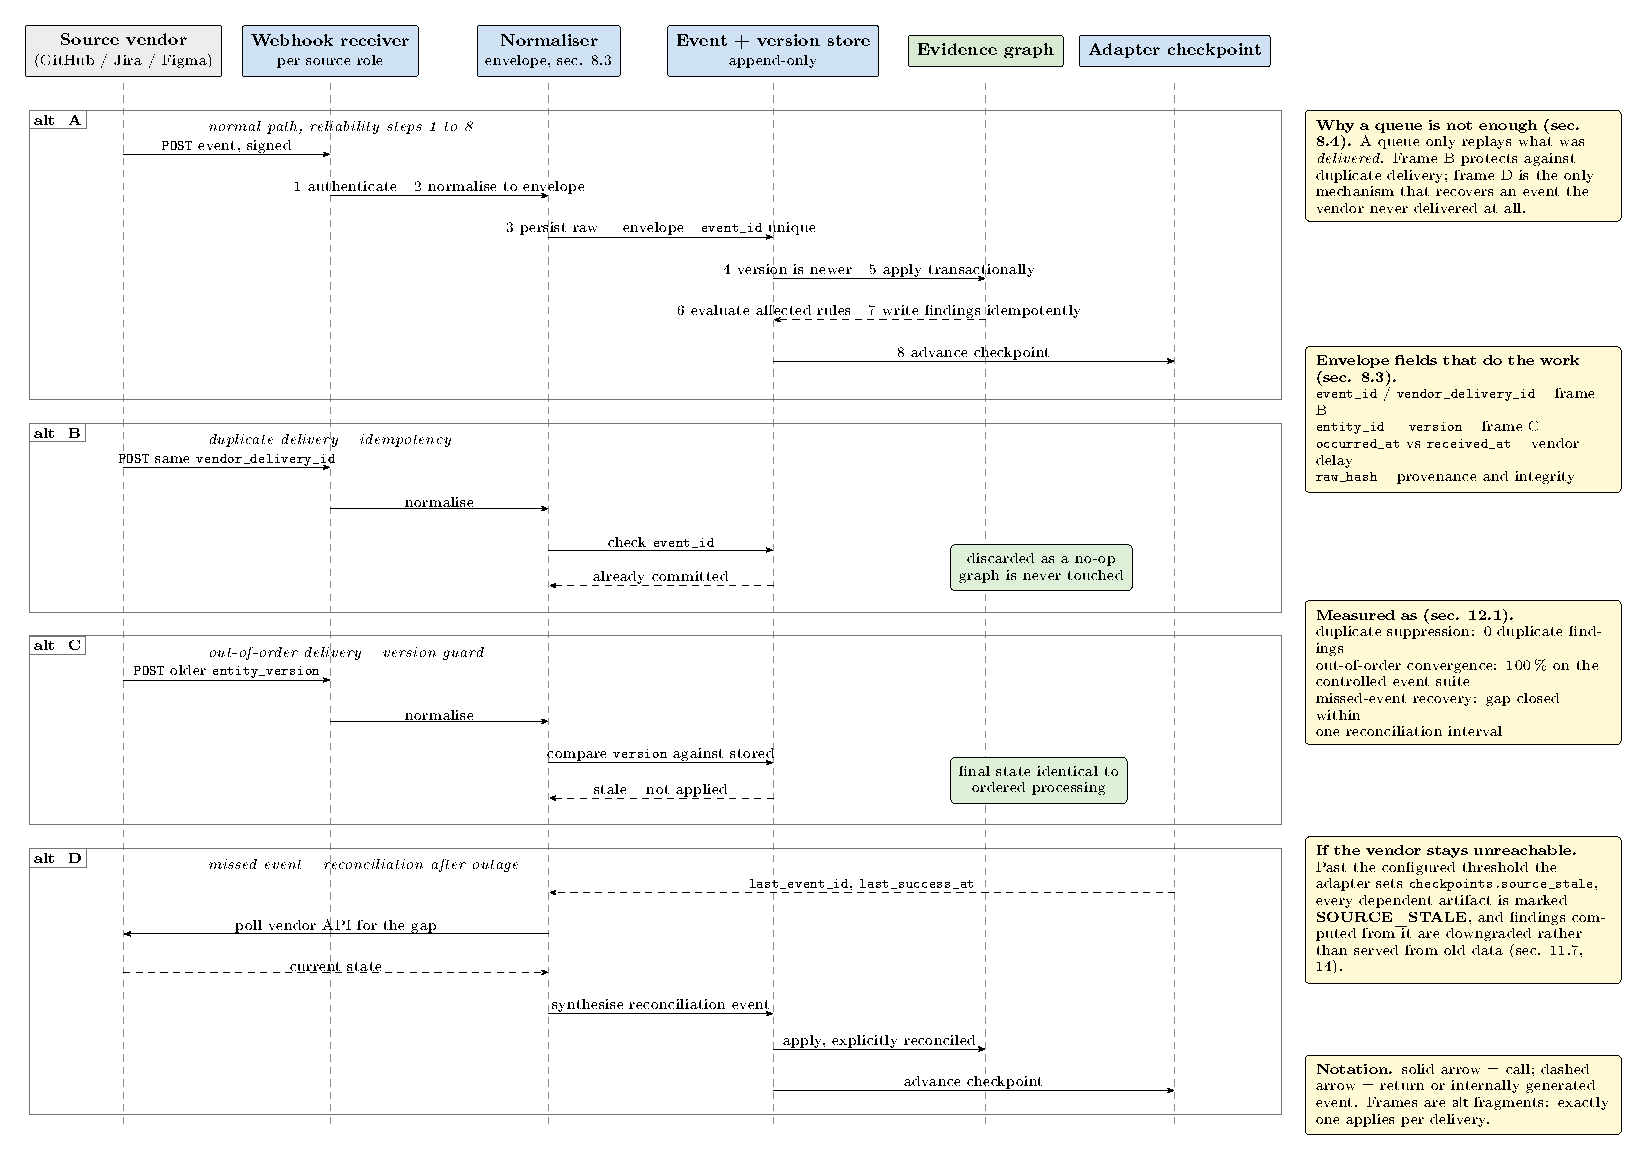
\includegraphics{diagrams/rendered/05_ingestion_sequence.pdf}}
  {Sequence diagram of source ingestion: one \textsf{alt} fragment covering
   first delivery, duplicate delivery, out-of-order delivery and missed-event
   reconciliation (proposal \S8.3--\S8.4).}
  {fig:ingestion-sequence}

\lsfigure{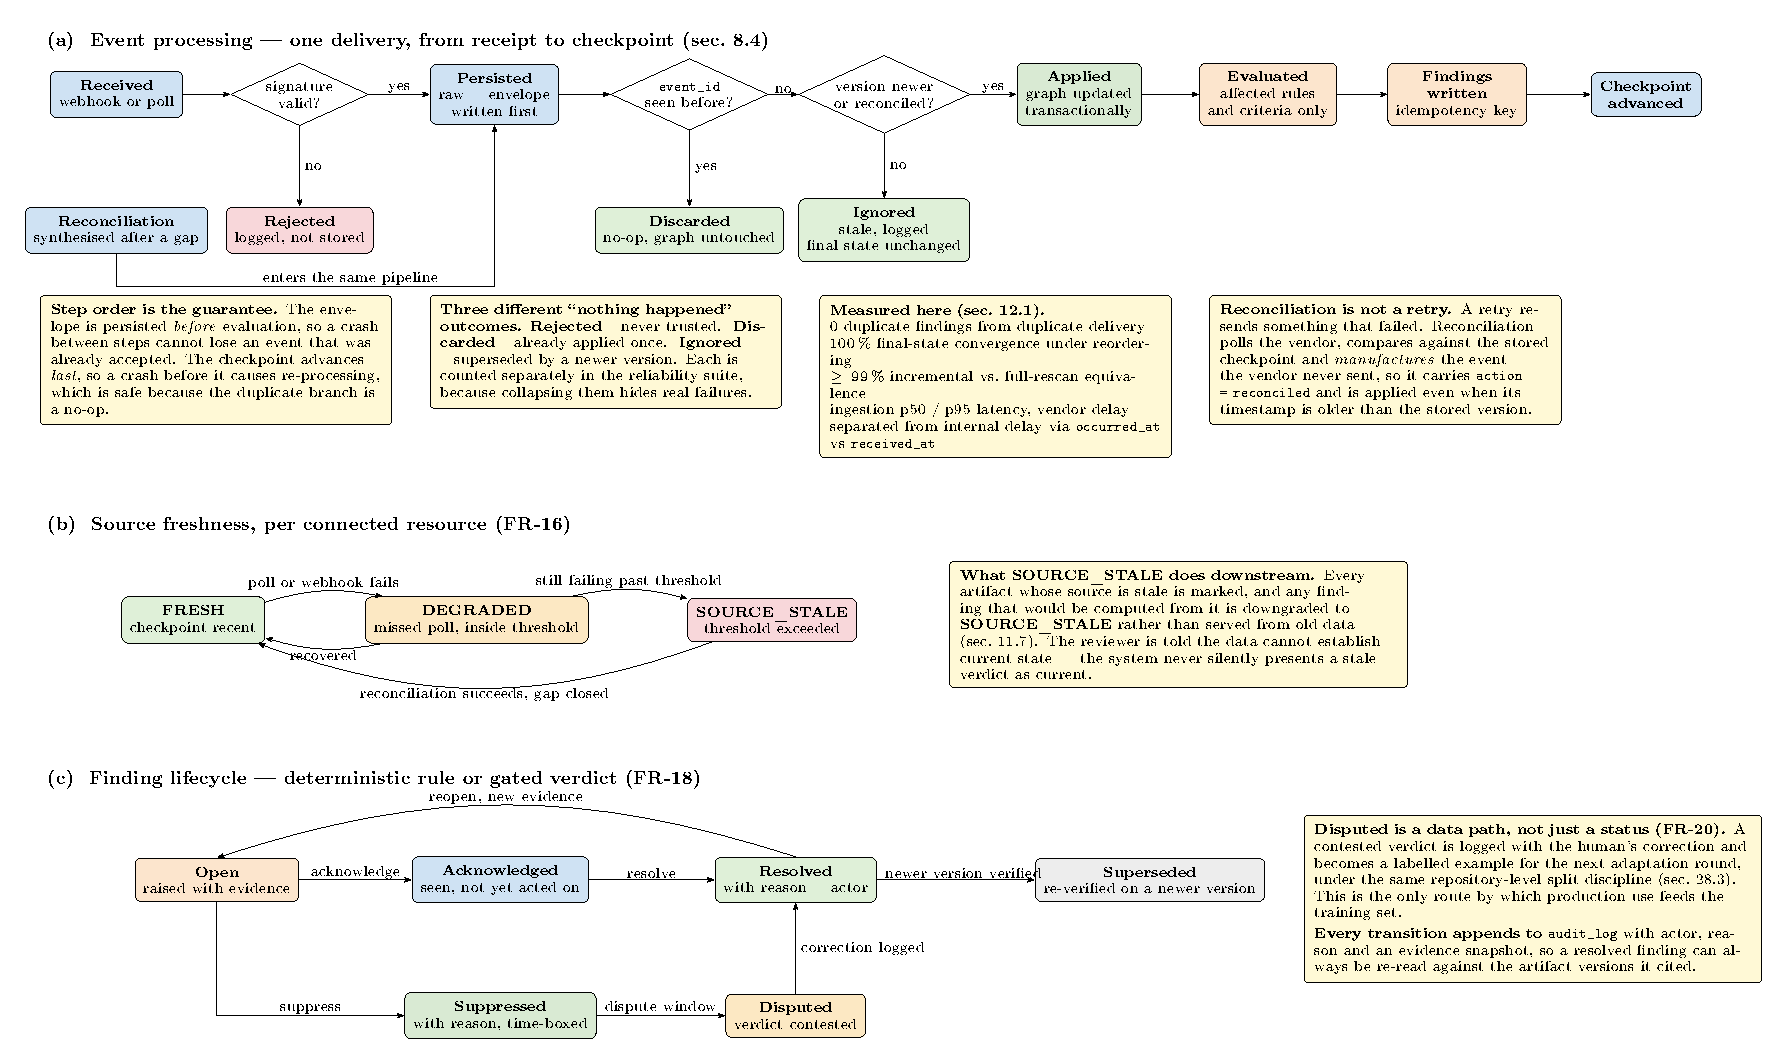
\includegraphics{diagrams/rendered/06_state_machines.pdf}}
  {State machines for (a) event processing, (b) source freshness (FR-16) and
   (c) the finding lifecycle (FR-18).}
  {fig:state-machines}

\lsfigure{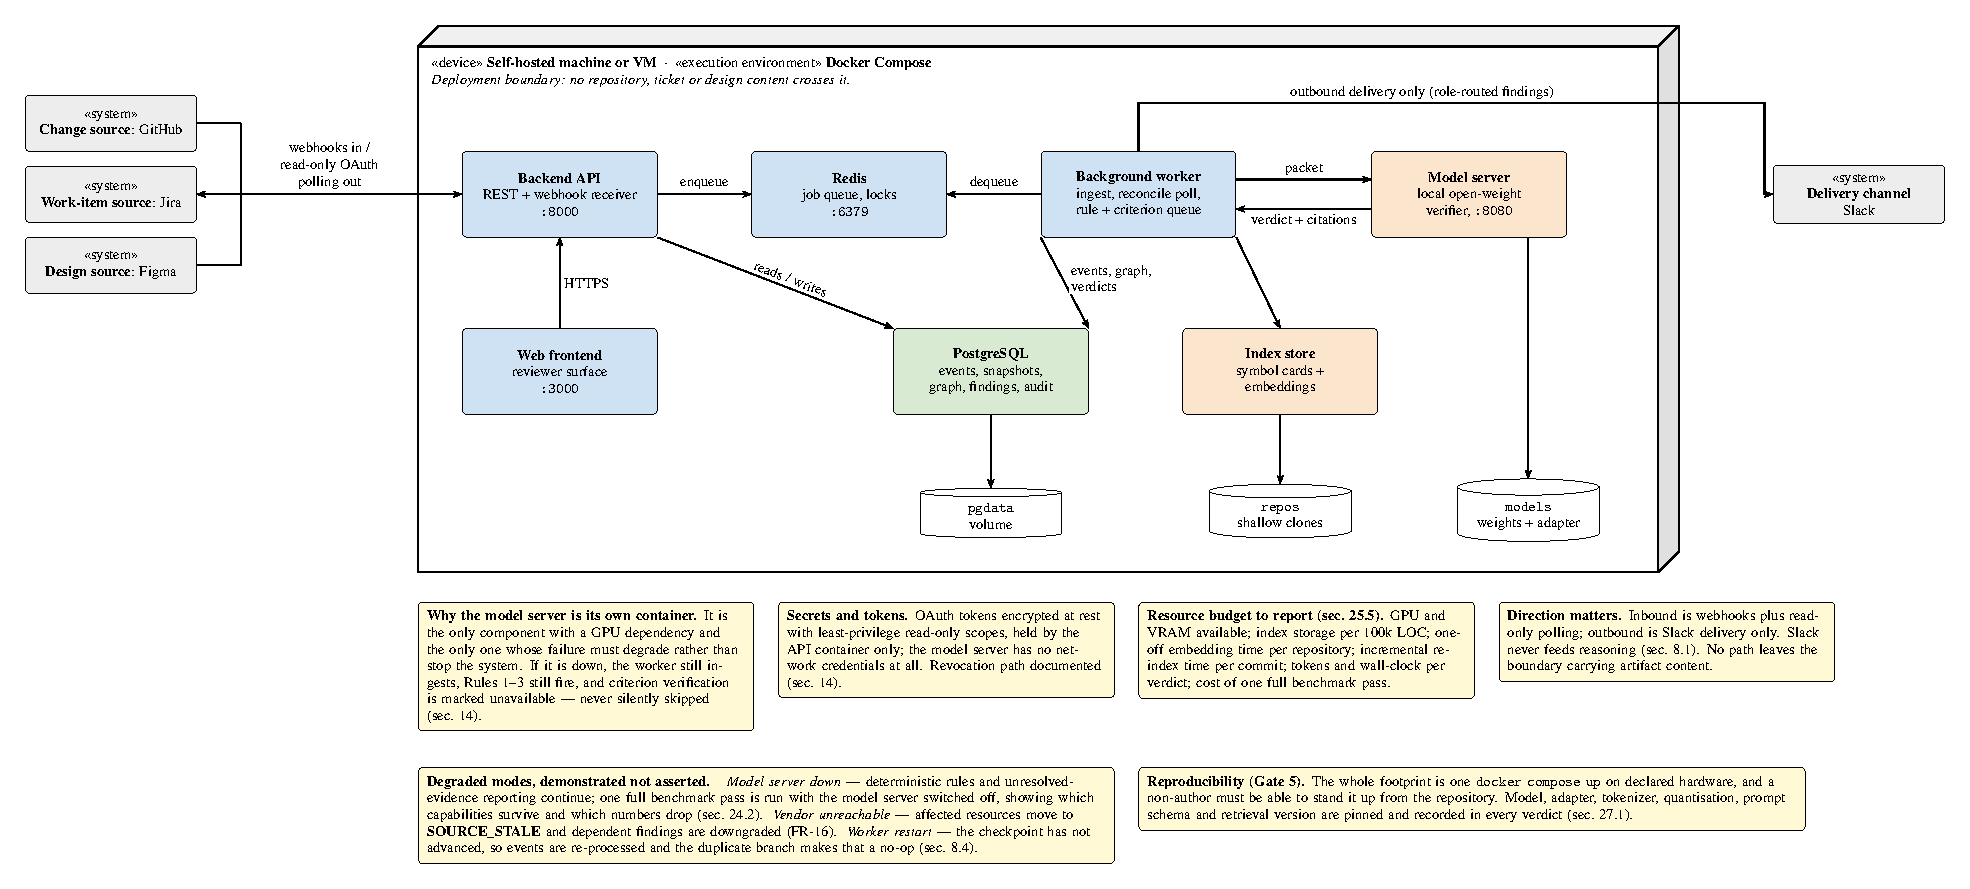
\includegraphics{diagrams/rendered/11_deployment.pdf}}
  {Deployment view: the single-host Docker Compose footprint, including the
   local model server, named volumes and the inbound/outbound boundary
   (proposal \S14).}
  {fig:deployment}
